\subsection{Shell以及环境变量}
\begin{frame}{``the Shell''}
    概念: 在计算机科学中, Shell俗称壳(用来区别于核),是指``为使用者提供操作界面''的\textcolor{red}{软件}。
    \begin{columns}
        \column{0.5\textwidth}
        \begin{myoutline}
            \1 图形界面 Shell
                \2 Graphical User Interface Shell, GUI Shell
                \2 Windows
                    \3 Windows Explorer
                \2 Linux
                    \3 X-Window
                    \3 GENOME
                    \3 \dots
        \end{myoutline}
        \column{0.5\textwidth}
        \begin{myoutline}
            \1 命令行 Shell
                \2 Command Line Interface Shell, CLI Shell
                \2 Windows
                    \3 CMD
                    \3 PowerShell
                \2 Linux
                    \3 sh
                    \3 bash
                    \3 zsh
                    \3 \dots
        \end{myoutline}
    \end{columns}

    \tiny{传统意义上的 Shell 指的是命令行式的 Shell}

    \tiny{Shell 是一个操作界面, 里面的每一个命令是怎么来的?}
\end{frame}

% 接下来,我将为大家再正式地总结一下,我们多次提到的 Shell 概念,
% 其实前面的讲解中,我们一直没以一个概念的形式向大家展示 Shell 是什么,而是让大家去使用 Shell,去感受它是什么
% 那么其实大家应该已经有一个概念了,
% 也就是幻灯片所述的,在计算机科学中, Shell俗称壳(用来区别于核),
% 是指``为使用者提供操作界面''的软件
% 其实计算机系统发展到现在, Shell 被分为两大类
% 一个是图形界面的 Shell, 可以用鼠标点点点的,适合所有人使用, 比如 Windows 的文件浏览器,或者 Ubuntu 的 GENOME 图形界面
% 更传统上的是命令行界面的 Shell, 我们刚刚讲的,和练习的,都是命令行的 Shell
% 我们在 Windows 的 PowerShell, Ubuntu 的 bash, MacOS 的 zsh 中进行了练习

% 虽然广义上讲,为用户提供操作界面的软件就是 Shell, 
% 也就是说类似 Windows 的文件浏览器或者其他鼠标点点点就完成操作的这种界面也是 Shell,
% 但是, 大家基本上不这么说, 大家说的 Shell, 默认还是指的传统的命令行 Shell

% 那讲到这儿其实就引出了一个问题, 我们使用的 Shell, 它给我们提供了这么多命令和功能,
% 那这些命令是什么, 怎么来的呢?

\begin{frame}{命令与PATH}
    PATH是一个环境变量, PATH 中包含了\textcolor{red}{可执行文件} 的搜索路径

    \begin{columns}
        \column{0.5\textwidth}
            \tiny{
            当要求系统运行一个程序而没有告诉它程序所在的完整路径时,
            系统除了在当前目录下面寻找此程序外,还应到``PATH''中指定的路径去找。
            用户通过设置环境变量, 来更好的运行进程。
            }
        \column{0.5\textwidth}
        \begin{figure}
            \begin{flushright}
                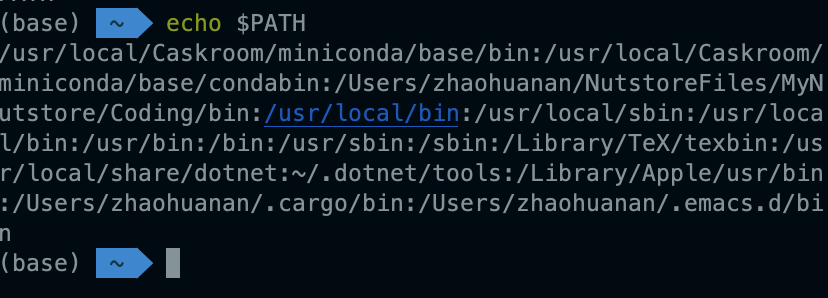
\includegraphics[width=1\linewidth]{Images/path.jpg}
            \end{flushright}
        \end{figure}
    \end{columns}
\end{frame}


\begin{frame}[standout]{PATH 的演示}
    \begin{myoutline}
        \1 MacOS/Linux
            \2 \$PATH
        \1 Windows
            \2 \%PATH\%
    \end{myoutline}
\end{frame}

% Windows 演示
% echo %PATH%
% C:\Windows\system32;C:\Windows;C:\Windows\System32\Wbem;C:\Windows\System32\W
% indowsPowerShell\v1.0\;C:\Windows\System32\OpenSSH\;C:\ProgramData\chocolatey
% \bin;C:\Program Files\OpenSSH-Win64;C:\opscode\chef\bin\;C:\Windows\system32\
% config\systemprofile\AppData\Local\Microsoft\WindowsApps;C:\Users\vagrant\sco
% op\shims_;C:\Users\vagrant\AppData\Local\Microsoft\WindowsApps;

% where python
% C:\Users\vagrant\AppData\Local\Microsoft\WindowsApps\python.exe

% 注释掉 Python 的 app path
% where python
% 找不着
% 再该回来
% where python
% 找到了

% MacOS 演示
% (base)  ~  PATH=/usr/local/Caskroom/miniconda/base/bin:/usr/local/Caskroom/miniconda/base/condabin:/Users/zhaohuanan/NutstoreFiles/MyNutstore/Coding/bin:/usr/local/bin:/usr/local/sbin:/usr/local/bin:/usr/bin:/bin:/usr/sbin:/sbin:/Library/TeX/texbin:/usr/local/share/dotnet:~/.dotnet/tools:/Library/Apple/usr/bin:/Users/zhaohuanan/.cargo/bin
% (base)  ~  which doom
% doom not found
% (base)  ✘  ~  PATH=/usr/local/Caskroom/miniconda/base/bin:/usr/local/Caskroom/miniconda/base/condabin:/Users/zhaohuanan/NutstoreFiles/MyNutstore/Coding/bin:/usr/local/bin:/usr/local/sbin:/usr/local/bin:/usr/bin:/bin:/usr/sbin:/sbin:/Library/TeX/texbin:/usr/local/share/dotnet:~/.dotnet/tools:/Library/Apple/usr/bin:/Users/zhaohuanan/.cargo/bin
% (base)  ✘  ~  PATH=/usr/local/Caskroom/miniconda/base/bin:/usr/local/Caskroom/miniconda/base/condabin:/Users/zhaohuanan/NutstoreFiles/MyNutstore/Coding/bin:/usr/local/bin:/usr/local/sbin:/usr/local/bin:/usr/bin:/bin:/usr/sbin:/sbin:/Library/TeX/texbin:/usr/local/share/dotnet:~/.dotnet/tools:/Library/Apple/usr/bin:/Users/zhaohuanan/.cargo/bin:/Users/zhaohuanan/.emacs.d/bin
% (base)  ~  which doom
% /Users/zhaohuanan/.emacs.d/bin/doom


\begin{frame}{演示结论}
    \begin{myoutline}
        \1 我们使用的命令,其本质是可执行文件
            \2 可执行文件具有完整的路径
            \2 可以直接使用命令的名称, 是因为其所在文件目录在 PATH 中
        \1 通过 PATH 中添加路径, 可以省略可执行文件的完整路径
            \2 当系统找不到用户输入的可执行文件时, 会在 PATH 中从前到后查找
            \2 当在PATH 中所有的路径下都找不到用户的可执行文件,会报错没有此可执行文件
        \1 安装程序时, 可以将可执行文件目录加入 PATH, 以方便使用此程序
    \end{myoutline}
\end{frame}


% 读 ppt 即可
% 那么到这里我们在操作系统和编程语言这一小节中, 关于 Shell 以及环境变量的知识就讲完了

